%%%%%%%%%%%%%%%%%%%%%%%%%%%%%%%%%%%%%%%%%%
% Engineering problems / LaTeX Template
%		Semester 5
%		Institut d'Optique Graduate School
%%%%%%%%%%%%%%%%%%%%%%%%%%%%%%%%%%%%%%%%%%
%	6N-INum-BlockX	/ Digital conversion
%%%%%%%%%%%%%%%%%%%%%%%%%%%%%%%%%%%%%%%%%%
%
% Created by:
%	Julien VILLEMEJANE - 25/may/2024
% Modified by:
%	
%
%%%%%%%%%%%%%%%%%%%%%%%%%%%%%%%%%%%%%%%%%%
% Professional Newsletter Template
% LaTeX Template
% Version 1.0 (09/03/14)
%
% Created by:
% Bob Kerstetter (https://www.tug.org/texshowcase/) and extensively modified by:
% Vel (vel@latextemplates.com)
% 
% This template has been downloaded from:
% http://www.LaTeXTemplates.com
%
% License:
% CC BY-NC-SA 3.0 (http://creativecommons.org/licenses/by-nc-sa/3.0/)
%
%%%%%%%%%%%%%%%%%%%%%%%%%%%%%%%%%%%%%%%%%

\documentclass[10pt]{article} % The default font size is 10pt; 11pt and 12pt are alternatives

%%%%%%%%%%%%%%%%%%%%%%%%%%%%%%%%%%%%%%%%%
% Professional Newsletter Template
% Structural Definitions File
% Version 1.0 (09/03/14)
%
% Created by:
% Vel (vel@latextemplates.com)
% 
% This file has been downloaded from:
% http://www.LaTeXTemplates.com
%
% License:
% CC BY-NC-SA 3.0 (http://creativecommons.org/licenses/by-nc-sa/3.0/)
%
%%%%%%%%%%%%%%%%%%%%%%%%%%%%%%%%%%%%%%%%%

%----------------------------------------------------------------------------------------
%	REQUIRED PACKAGES
%----------------------------------------------------------------------------------------

\usepackage{graphicx} % Required for including images
\usepackage{microtype} % Improved typography
\usepackage{multicol} % Used for the two-column layout of the document
\usepackage{booktabs} % Required for nice horizontal rules in tables
\usepackage{wrapfig} % Required for in-line images
\usepackage{float} % Required for forcing figures not to float with the [H] parameter

%------------------------------------------------
% Fonts

\usepackage{charter} % Use the Charter font as the main document font
\usepackage{courier} % Use the Courier font for \texttt (monospaced) only
\usepackage[T1]{fontenc} % Use T1 font encoding
\usepackage{lmodern}

%------------------------------------------------
% List Separation

\usepackage{enumitem} % Required to customize the list environments
\setlist{noitemsep,nolistsep} % Remove spacing before, after and within lists for a compact look

%------------------------------------------------
% Figure and Table Caption Styles

\usepackage{caption} % Required for changing caption styles
\captionsetup[table]{labelfont={bf,sf},labelsep=period,justification=justified} % Specify the table caption style
\captionsetup[figure]{labelfont={sf,bf},labelsep=period,justification=justified, font=small} % Specify the figure caption style
\setlength{\abovecaptionskip}{10pt} % Whitespace above captions

%------------------------------------------------
% Spacing Between Paragraphs

\makeatletter
\usepackage{parskip}
\setlength{\parskip}{6pt}
\newcommand{\@minipagerestore}{\setlength{\parskip}{6pt}}
\makeatother

%----------------------------------------------------------------------------------------
%	PAGE MARGINS AND SPACINGS
%----------------------------------------------------------------------------------------

\textwidth = 7 in % Text width
\textheight = 10 in % Text height
\oddsidemargin = -18pt % Left side margin on odd pages
\evensidemargin = -18pt % Left side margin on even pages
\topmargin = -36pt % Top margin
\headheight = 0pt % Remove the header by setting its space to 0
\headsep = 0pt % Remove the space between the header and top of the page
\parskip = 4pt % Space between paragraph
\parindent = 0.0in % Paragraph indentation
\pagestyle{empty} % Disable page numbering

%----------------------------------------------------------------------------------------
%	COLORS
%----------------------------------------------------------------------------------------

\usepackage[dvipsnames,svgnames]{xcolor} % Required to specify custom colors

\definecolor{altncolor}{rgb}{.8,0,0} % Dark red
%\definecolor{altncolor}{rgb}{.2,.4,.8} % Dark blue
%\definecolor{altncolor}{rgb}{.84,.16,.16} % Red

\usepackage[colorlinks=true, linkcolor=altncolor, anchorcolor=altncolor, citecolor=altncolor, filecolor=altncolor, menucolor=altncolor, urlcolor=altncolor]{hyperref} % Use the color defined above for all links

%----------------------------------------------------------------------------------------
%	DRAWINGS & CIRCUITS
%----------------------------------------------------------------------------------------

\usepackage{tikz}
\usepackage{pgfplots}

\usepackage[european, straightvoltages]{circuitikz}
\usetikzlibrary{babel, patterns, patterns.meta, calc}

%----------------------------------------------------------------------------------------
%	PDF
%----------------------------------------------------------------------------------------

\usepackage{pdfpages}

%----------------------------------------------------------------------------------------
%	BOX STYLES
%----------------------------------------------------------------------------------------

\usepackage[framemethod=TikZ]{mdframed}% Required for creating boxes
\mdfdefinestyle{sidebar}{
    linecolor=black, % Outer line color
    outerlinewidth=0.5pt, % Outer line width
    roundcorner=0pt, % Amount of corner rounding
    innertopmargin=10pt, % Top margin
    innerbottommargin=10pt, % Bottom margin
    innerrightmargin=10pt, % Right margin
    innerleftmargin=10pt, % Left margin
    backgroundcolor=white, % Box background color
    frametitlealignment=\centering,
    frametitlebackgroundcolor=gray!20, % Title background color
    frametitlerule=false, % Title rule - true or false
    frametitlerulecolor=white, % Title rule color
    frametitlerulewidth=0.5pt, % Title rule width
    frametitlefont=\Large\bfseries, % Title heading font specification
    font=\small
}

\mdfdefinestyle{intextbox}{
    linecolor=black, % Outer line color
    outerlinewidth=0.5pt, % Outer line width
    roundcorner=10pt, % Amount of corner rounding
    innertopmargin=7pt, % Top margin
    innerbottommargin=7pt, % Bottom margin
    innerrightmargin=7pt, % Right margin
    innerleftmargin=7pt, % Left margin
    backgroundcolor=white, % Box background color
    frametitlealignment=\centering,
    frametitlebackgroundcolor=gray!20, % Title background color
    frametitlerule=false, % Title rule - true or false
    frametitlerulecolor=white, % Title rule color
    frametitlerulewidth=0.5pt, % Title rule width
    frametitlefont=\Large\bfseries % Title heading font specification
}

\mdfdefinestyle{aavbox}{
    linecolor=black, % Outer line color
    outerlinewidth=0.2pt, % Outer line width
    roundcorner=5pt, % Amount of corner rounding
    innertopmargin=7pt, % Top margin
    innerbottommargin=7pt, % Bottom margin
    innerrightmargin=7pt, % Right margin
    innerleftmargin=7pt, % Left margin
    backgroundcolor=gray!10, % Box background color
    frametitlealignment=\centering,
    frametitlebackgroundcolor=gray!30, % Title background color
    frametitlerule=false, % Title rule - true or false
    frametitlerulecolor=white, % Title rule color
    frametitlerulewidth=0.2pt, % Title rule width
    frametitlefont=\Large\bfseries % Title heading font specification
}

%----------------------------------------------------------------------------------------
%	HEADING STYLE
%----------------------------------------------------------------------------------------

\newcommand{\heading}[2]{ % Define the \heading command
\vspace{#2} % White space above the heading
{\begin{center}\Large\textbf{#1}\end{center}} % The heading style
\vspace{#2} % White space below the heading
}

\newcommand{\BackToContents}{\hyperlink{contents}{{\small Back to Contents}}} % Define a command for linking back to the contents of the newsletter

\usepackage{listings}
\lstset{language = Python, 
	basicstyle={\small \color{black}}, 
	tabsize = 3,
	commentstyle=\color{black!70!green},
	linewidth=160mm,
	framexleftmargin=5mm, frame=shadowbox, rulesepcolor=\color{black},
  	numbers=left,
	xleftmargin=40pt,
	escapechar=|
} % Include the document which specifies all packages and structural customizations for this template
\usepackage{amsmath}

%----------------------------------------------------------------------------------------
%	DOCUMENT INFORMATIONS
%----------------------------------------------------------------------------------------
\def\module{Interfaçage Numérique}
\def\submodule{Interfaçage Numérique}
\def\moduleSmall{6N-047-SCI / INum}
\def\year{2024-2025}
\def\problem{Bloc X - Conversion Numérique}
\def\problemName{Piloter et transmettre en numérique}

\def\validation{}

\def\scheduleCM{0}
\def\scheduleTD{2}
\def\scheduleTDcomputer{0}
\def\scheduleTP{0}

\def\workingTeam{En groupe}

\def\workingSpecial{}

\def\keywords{Moteurs; PWM; Codage des informations; Transmission d'information}


\begin{document}
%----------------------------------------------------------------------------------------
%	HEADER IMAGE
%----------------------------------------------------------------------------------------

\begin{figure}[H]
\centering
\includegraphics[width=0.5\linewidth]{../../../../_assets/latex/logo_iogs.png}
\end{figure}

%----------------------------------------------------------------------------------------
%	SIDEBAR - FIRST PAGE
%----------------------------------------------------------------------------------------

\begin{minipage}[t]{.33\linewidth} % Mini page taking up 30% of the actual page
\begin{mdframed}[style=sidebar,frametitle={\module}] % Sidebar box

%-----------------------------------------------------------
%	DOCUMENT DESCRIPTION
\begin{center}

\textit{\large \centering \year}
\end{center}


\centerline {\rule{.70\linewidth}{.25pt}} % Horizontal line

\begin{center}
	\textit{\large \moduleSmall}
\end{center}

\centerline {\rule{.70\linewidth}{.25pt}} % Horizontal line

\begin{center}
	\textbf{\problem} ( \validation )
\end{center}

\centerline {\rule{.70\linewidth}{.25pt}} % Horizontal line

%-----------------------------------------------------------

\textbf{Concepts étudiés}

\begin{itemize}
\item[\textsc{\scriptsize [Phys]}] Moteur et champs électriques
\item[\textsc{\scriptsize [Num]}] Modulation de largeur d'impulsion
\item[\textsc{\scriptsize [Num]}] Codage des informations
\item[\textsc{\scriptsize [Num]}] Transmission des informations
\end{itemize}

\centerline {\rule{.70\linewidth}{.25pt}} % Horizontal line

%-----------------------------------------------------------

\textbf{Mots clefs}

\keywords

\centerline {\rule{.70\linewidth}{.25pt}} % Horizontal line

%-----------------------------------------------------------

\textbf{Sessions}

\begin{itemize}
\item[\textbf{\scheduleCM}] Cours(s) - 1h30
\item[\textbf{\scheduleTD}] TD(s) - 1h30
\item[\textbf{\scheduleTDcomputer}] TD(s) Machine - 2h00
\item[\textbf{\scheduleTP}] TP(s) - 4h30
\end{itemize}

\centerline {\rule{.70\linewidth}{.25pt}} % Horizontal line

{\large Travail}

\textbf{\workingTeam}

\textbf{\workingSpecial}

%-----------------------------------------------------------
\end{mdframed}


\begin{minipage}[t]{.95\linewidth}
\textbf{Institut d'Optique}\\
Graduate School, \textit{France}\\
\href{https://www.institutoptique.fr}{https://www.institutoptique.fr}

\medskip
\textbf{GitHub - Digital Methods}

\href{https://github.com/IOGS-Digital-Methods}{https://github.com/IOGS-Digital-Methods}

\end{minipage}

\end{minipage}\hfill % End the sidebar mini page 
% NO SPACE BETWEEN THE END OF SIDEBAR AND BEGIN OF MAIN PART
%----------------------------------------------------------------------------------------
%	MAIN BODY - FIRST PAGE
%----------------------------------------------------------------------------------------
%
\begin{minipage}[t]{.65\linewidth} % Mini page taking up 65% of the actual page

\hypertarget{context}{\heading{\huge \problemName}{6pt}} % \hypertarget provides a label to reference using \hyperlink{label}{link text}

\centerline {\rule{.70\linewidth}{.25pt}} % Horizontal line

%% Short introduction 
BLA BLA BLA BLA

%%

\bigskip

%----------------------------------------------------------------------------------------
%	IN-TEXT BOX / Intended learning outcomes
%----------------------------------------------------------------------------------------

\begin{mdframed}[style=aavbox,frametitle={Acquis d'Apprentissage Visés}]

En résolvant ces problèmes, les étudiant$\cdot$e$\cdot$s seront capables de  :

\centerline {\rule{.40\linewidth}{.1pt}} % Horizontal line

\begin{center}
{\large \textsc{Côté Numérique}}
\end{center}

\begin{enumerate}
\item \textbf{Générer des signaux numériques} permettant le pilotage de moteurs
\item \textbf{Lister les différentes informations numériques et leur codage}
\item \textbf{Transcoder des informations numériques} pour leur transmission numérique
\end{enumerate}

\centerline {\rule{.40\linewidth}{.1pt}} % Horizontal line

\begin{center}
{\large \textsc{Côté Physique}}
\end{center}

\begin{enumerate}
\item \textbf{Comprendre le principe de fonctionnement d'un moteur} à courant continu et pas à pas
\item \textbf{Comprendre l'intérêt des étages de puissance} dans le pilotage numérique
\end{enumerate}

\end{mdframed}

%-----------------------------------------------------------


\medskip

%\begin{wrapfigure}[7]{l}[0pt]{0pt} % In-line figure with text wrapping around it
%\includegraphics[width=0.3\textwidth]{engPb_S5_01/placeholder.jpg}
%\end{wrapfigure}

\end{minipage} % End the main body - first page mini page

%----------------------------------------------------------------------------------------
%	MAIN BODY - SECOND PAGE
%----------------------------------------------------------------------------------------
\newpage

%-----------------------------------------------------------

\hypertarget{stepbystep}{\heading{Séance 1 / Moteurs et pilotage numérique}{6pt}} % \hypertarget provides a label to reference using \hyperlink{label}{link text}

\centerline {\rule{.70\linewidth}{.25pt}} % Horizontal line
%-----------------------------------
\section*{Moteurs à courant continu / Modélisation}

\centerline {\rule{.70\linewidth}{.25pt}} % Horizontal line

%%%%%%%%%%%%%%%%%%%%%%%%%%%%%%%
\subsection*{Modèle d'un moteur à courant continu}

Il est possible de modéliser électriquement et mécaniquement un moteur à courant continu de la façon suivante :

\begin{center}
	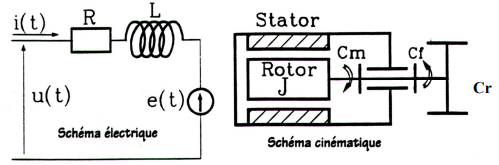
\includegraphics{images/moteur_elec_meca.png}
\end{center}
\textit{\small Source : http://s2i.chaptal.free.fr/ }

Un moteur est un élément permettant de convertir une puissance électrique en une puissance mécanique. 
Le couple ($C_m$) est lié au courant ($I$) par une constante intrinsèque au moteur, notée $K$ : 
$$C_m = K \cdot I$$

La vitesse de rotation ($\Omega$) est liée à la tension aux bornes du moteur ($U$) par cette même constante : 
$$E = K \cdot \Omega$$

La puissance électrique (ou mécanique) vaut : $P_e = C \cdot \Omega = E \cdot I$

D'après le principe fondamental de la dynamique, il existe un lien entre le couple appliqué sur le rotor du moteur et la vitesse de rotation :

$$C_m - C_R - f \cdot \Omega = J \cdot p \cdot \Omega$$

où $C_r$ correspond au couple résistant, $f$ au coefficient de frottement visqueux, $J$ à l'inertie du moteur. 

En reliant toutes ces équations, on peut obtenir la fonction de transfert entre la vitesse de rotation du système ($\Omega$) et la tension appliquée sur le stator ($U$) suivante : 

$$H(p) = \frac{\Omega(p)}{U(p)} = \frac{K}{(J \cdot p + f) \cdot (R + L \cdot p) + K^2}$$


%%%%%%%%%%%%%%%%%%%%%%%%%%%%%%%
\subsection*{Exemple du moteur POLOLU 3239}

\begin{center}
	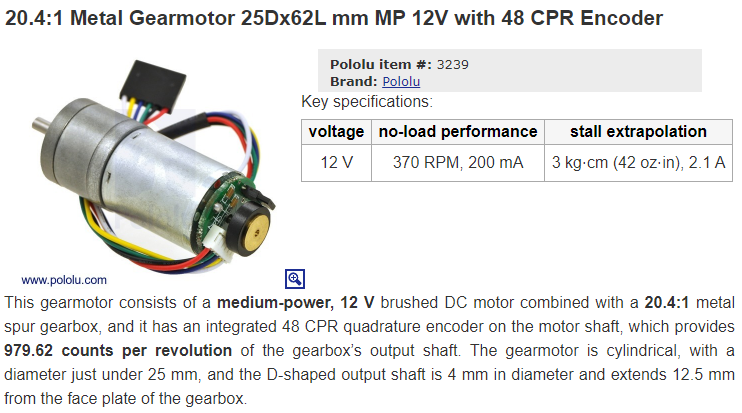
\includegraphics[width=11cm]{images/POL3239_2.png}
\end{center}

\begin{enumerate}
	\item Quels sont les paramètres importants à prendre en compte ?
	\item Les valeurs anoncées sont-elles cohérentes ?

	\item Quelle est la valeur du coefficient $K$, lien entre la vitesse de rotation et la tension aux bornes du moteur ?	
\end{enumerate}

\begin{center}
	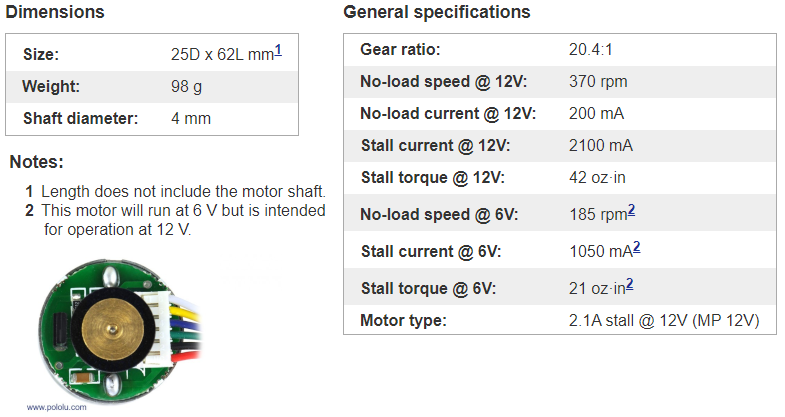
\includegraphics[width=11cm]{images/POL3239_1.png}
\end{center}


%%%%%%%%%%%%%%%%%%%%%%%%%%%%%%%
\subsection*{Modèle simplifié d'un MCC}

Il est possible de simplifier le modèle précédent, en faisant l'hypothèse que le temps de réponse de la partie électrique (dont la constante de temps sera notée $\tau_e$) est plus petit que le temps de réponse mécanique (dont la constante de temps sera notée $\tau_m$).

$$H(p) = \frac{K_0}{(1 + \tau_m \cdot p) \cdot (1 + \tau_e \cdot p)}$$

Avec $\tau_m = R \cdot J / (K^2 + R \cdot f)$, $\tau_e = L / R $ et $K_0 = K / (K^2 + R \cdot f)$

\medskip

\begin{enumerate}
	\item Cette hypothèse est-elle vérifiée si on prend comme valeurs : $K = 0.1\operatorname{Nm/A}$ (ou en V/rd/s), $J = 0.01\operatorname{jg.m^2}$, $L = 0.5\operatorname{mH}$ et $R = 0.1\operatorname{\Omega}$ (en absence de frottement) ?
	\item Ce système est-il stable ?
	\item Parmi les réponses indicielles suivantes, laquelle correspond à ce système ?
	
	\begin{center}
		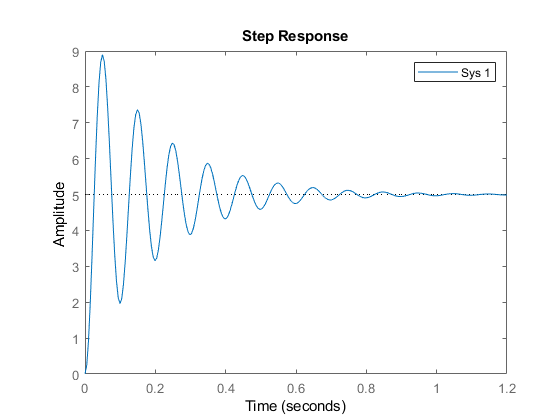
\includegraphics[width=6cm]{images/moteur_sys1.png}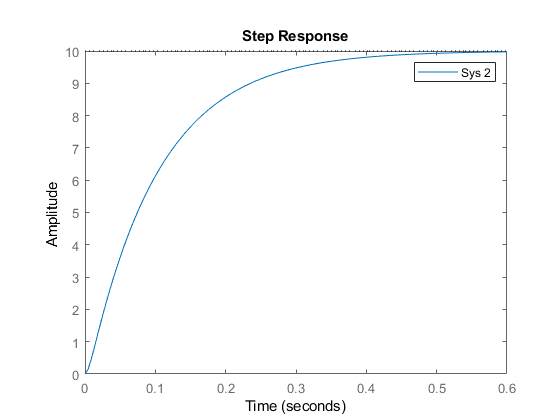
\includegraphics[width=6cm]{images/moteur_sys2.png}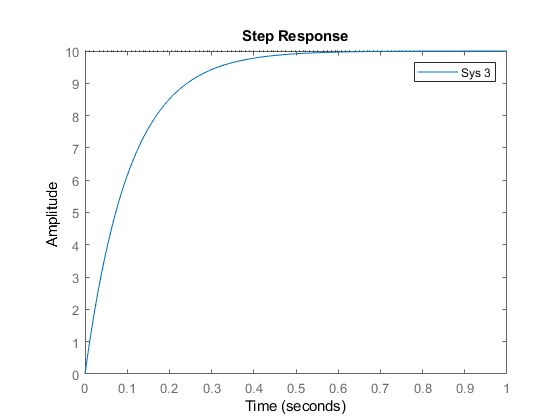
\includegraphics[width=6cm]{images/moteur_sys3.png}
	\end{center}
\end{enumerate}


\centerline {\rule{.70\linewidth}{.25pt}} % Horizontal line
%-----------------------------------
\section*{Moteurs à courant continu / Pilotage en vitesse}

\centerline {\rule{.70\linewidth}{.25pt}} % Horizontal line

\subsection*{Variation analogique de la vitesse de rotation}

Proposez une solution pour pouvoir piloter analogiquement ce système en vitesse : (a) dans un sens, (b) dans les deux directions.

%%%%%%%%%%%%%%%%%%%%%%%%%%%%%%%
\subsection*{Variation numérique de la vitesse de rotation}

On se propose à présent de piloter ce système de manière numérique. 

\begin{enumerate}
	\item Comment est-il possible de faire varier la vitesse de rotation numériquement ?
	\item Quel est l'intérêt d'un tel mode de fonctionnement ?
	\item Proposez un montage, basé sur le pilotage par carte Nucléo, d'un MCC dans une direction.
	\item Proposez un programme pour le pilotage par carte Nucléo d'un MCC dans une direction.	
	\item Comment est-il possible de piloter ce MCC dans les deux sens de rotation ?
	
	On se propose d'utiliser le composant L293D (voir partie de la documentation technique en annexe).
	
	\item Proposez un montage, basé sur le pilotage par carte Nucléo, d'un MCC dans les deux directions.
	\item Proposez un programme pour le pilotage par carte Nucléo d'un MCC dans les deux directions.
\end{enumerate}


\centerline {\rule{.70\linewidth}{.25pt}} % Horizontal line
%-----------------------------------
\section*{Mesure de vitesse}

\centerline {\rule{.70\linewidth}{.25pt}} % Horizontal line


\begin{enumerate}
	\item Proposez une solution de mesure de vitesse de rotation.
	
	On se propose d'utiliser un encodeur tel que proposé dans la figure suivante :
	
\begin{center}
	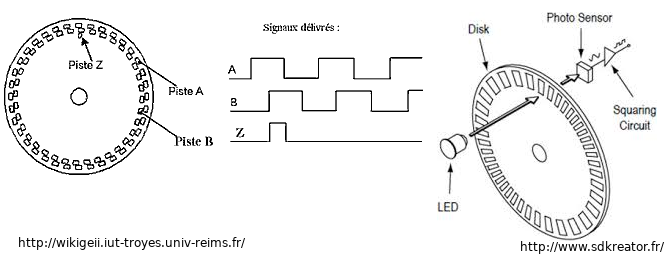
\includegraphics[width=10cm]{images/encodeur_optique_AB.png}
\end{center}	
	
	\item Proposez une méthode pour mesurer la vitesse de rotation.	
	\item Comment connaître le sens de rotation ? La position ?
\end{enumerate}


\centerline {\rule{.70\linewidth}{.25pt}} % Horizontal line
%-----------------------------------
\section*{Moteurs pas à pas / Principe et pilotage}

\centerline {\rule{.70\linewidth}{.25pt}} % Horizontal line

%%%%%%%%%%%%%%%%%%%%%%%%%%%%%%%
\subsection*{Principe de fonctionnement d'un moteur pas à pas}

Un moteur pas à pas est constitué de 2 bobines séparées d'un certain angle. En alimentant indépendamment les deux bobines, on vient modifier la direction du champ magnétique résultant.

\begin{center}
	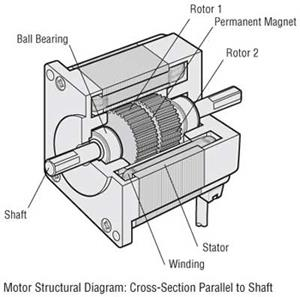
\includegraphics[width=5cm]{images/moteur_pas_pas.png}
\end{center}

Pour avancer d'un pas, il suffit alors de suivre le protocole suivant : 

\begin{center}
	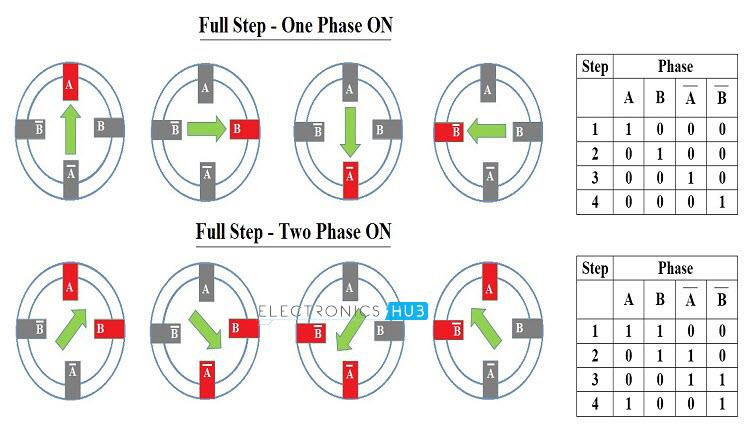
\includegraphics[width=10cm]{images/moteur_pas_cmd.png}
\end{center}

\begin{enumerate}
	\item Quel est l'intérêt d'un tel moteur ?
	\item Comment le faire tourner dans l'autre sens ?
	\item Quel est l'intérêt du deuxième mode de fonctionnement proposé ?
	\item Peut-on combiner les deux ?
\end{enumerate}

%%%%%%%%%%%%%%%%%%%%%%%%%%%%%%%
\subsection*{Pilotage numérique}

\begin{enumerate}
	\item Proposez un câblage pour pouvoir piloter ce moteur pas à pas à l'aide du pont en H L293D.
	\item Proposez un programme pour le pilotage par carte Nucléo d'un moteur pas à pas dans les deux directions.
\end{enumerate}


\centerline {\rule{.70\linewidth}{.25pt}} % Horizontal line
%----------------------------------------------------------------------------------------



%----------------------------------------------------------------------------------------
%	MAIN BODY - SECOND PAGE
%----------------------------------------------------------------------------------------
\newpage

%-----------------------------------------------------------

\hypertarget{stepbystep}{\heading{Séance 2 / Transmission de données numériques}{6pt}} % \hypertarget provides a label to reference using \hyperlink{label}{link text}

\centerline {\rule{.70\linewidth}{.25pt}} % Horizontal line
%-----------------------------------
\section*{Exercices préliminaires}

\centerline {\rule{.70\linewidth}{.25pt}} % Horizontal line

%%%%%%%%%%%%%%%%%%%%%%%%%%%%%%%
\subsection*{Codage des informations}

On donne le codage hexadécimal du nombre réel $3.1418$ stocké dans une variable de type \textbf{float} : 0x( 40 13 49 40 ).

Cette conversion est basée sur la norme IEEE754 simple précision.

\begin{enumerate}
	\item Combien d'octets sont-ils nécessaires pour stocker cette information sous forme d'une variable de type \textbf{float} ?
	\item Combien d'octets sont-ils nécessaires pour stocker cette information sous forme d'une chaîne de caractères (type \textbf{char[]}) ?
	
	On stocke à présent cette donnée dans une variable de type \textbf{char} de la manière suivante : 
	\begin{verbatim}
		c = 3.1418;
	\end{verbatim}
	 	
	
	\item Que stocke la variable \textbf{c} ?
	\item Comment transférer la valeur réelle de ce nombre par l'intermédiaire de 4 octets en C++ ? En Python ?
\end{enumerate}


\centerline {\rule{.70\linewidth}{.25pt}} % Horizontal line
%%%%%%%%%%%%%%%%%%%%%%%%%%%%%%%
\subsection*{???}

Données sur 16 bits, mais on ne souhaite conserver que 8 bits.

On souhaite à présent transférer l'un après l'autre les 8 bits de poids forts puis les 8 bits de poids faibles.

\centerline {\rule{.70\linewidth}{.25pt}} % Horizontal line
%-----------------------------------
\section*{Contexte}

\centerline {\rule{.70\linewidth}{.25pt}} % Horizontal line

Un robot est équipé de deux roues motorisées indépendantes, ainsi que d'une roue folle. Les moteurs utilisés sont des moteurs à courant continu. Le robot possède également 2 phares sous forme de LEDs de puissance.

Une télécommande est associée à ce robot. Elle contient un joystick sur 2 axes (chacun des axes correspond à un potentiomètre qui fournit une tension analogique proportionnelle à la position) et 2 boutons-poussoirs pour : (1) démarrer ou arrêter le robot, (2) allumer ou éteindre les phares. 

SCHEMA DE PRINCIPE

\centerline {\rule{.70\linewidth}{.25pt}} % Horizontal line
%-----------------------------------
\section*{Transmission d'informations}

\subsection*{Utilisation d'un protocole série "simple"}

On souhaite mettre en place un protocole de communication permettant d'échanger des informations entre le robot et la télécommande.

Dans un premier temps, on s'intéressera à une liaison série de type RS232 à 115200 bauds, permettant de transmettre des octets de manière asynchrone.

Vous devez établir un protocole de communication permettant la réception par le robot des ordres de pilotage : démarrer/arrêter, allumer/éteindre les phares, avancer, reculer, s'arrêter... La vitesse d'avance du robot sera \textbf{constante}.

\subsection*{Utilisation d'un protocole série "avancé"}

La liaison série utilisée sera la même que précédemment.

Vous devez établir un protocole de communication permettant la réception par le robot des ordres de pilotage : démarrer/arrêter, allumer/éteindre les phares, avancer, reculer, s'arrêter... La vitesse d'avance du robot sera \textbf{proportionnelle} à la position du joystick (de même que la rotation).


\subsection*{Utilisation d'un module de transmission spécifique}



\end{document} 